\chapter{Návrh vylepšení systému}
\label{Návrh vylepšení systému}
V této kapitole jsou navrženy způsoby vylepšení navrženého systému.


% \section{Možnosti odstranění omezení navržené gatewaye - závislost na znalosti typu koncových zařízení senzorové sítě}
\section{Vylepšení infrastruktury systému}
Jedním z největších omezení navrženého systému je, že FW gatewaye musí podporovat typy koncových zařízení senzorové sítě, aby na základě typu koncového zařízení byl správně zpracován jeho payload.
Přidání nového typu zařízení do sítě vyžaduje update FW gatewaye.
Aby gateway nebyla závislá na znalosti typu koncových zařízení senzorové sítě, je potřeba přenášet celý aplikační payload koncových zařízení přes síť RS485, což má nežádoucí důsledek a to zvýšení objemu přenášených dat v síti RS485 přístupového systému.
Původní navržené řešení viz. kapitola \ref{Návrh senzorové sítě} totiž klade důraz na nízký objem přenášených dat v síti RS485.

Například použitý typ koncového zařízení RHF1S001 \ref{sec:RHF1S001} odesílá LoRaWAN pakety o délce 22 bytů, z toho je 9 bytů aplikační payload. Protokol umožňuje posílat pakety o velikosti až 256 bytů, z toho je nejméně 13 bytů data protokolu, tedy maximální délka aplikačního payloadu může být až 243 bytů.

Efektivní řešení by bylo rozšíření CKP protokolu sítě RS485 přístupového sytému o nový typ příkazu umožňující odeslat paket o maximální délce payloadu až 243 bytů, tedy aby jedním tímto paketem bylo možné odeslat celý aplikační payload. 
Je zde bezpečnostní výhoda, že aplikační payload by pak mohl být dešifrován až na serveru LoRaWAN klíčem AppSKey, tudíž data z koncových zařízení by nebyla odhalitelná v síti RS485.
Toto řešení tedy vyžaduje update FW všech kontrolních panelů, což je velmi náročné.
% tudíž realizace tohot řešení prozatím neni plánována.

Nicméně je možné implementovat podobné řešení bez nutnosti zavádění nového typu paketu pro aplikační payload koncového zařízení senzorové sítě tak, že aplikační payload by byl rozdělen a odeslán posloupností několika paketů průchod. 
Např. z dostupných 6 bytů v jednom paketu průchod by jeden byte obsahoval informaci o čísle paketu dané sekvence a zbylých 5 bytů by byly data payloadu daného koncového zařízení Zařízení typu RHF1S001, které má aplikační payload o velikosti 9 bytů by byl takto odeslán dvěma pakety průchod. Jelikož každý paket průchod je potvrzován, toto řešení by rapidně zvýšilo objem přenášených dat v síti RS485.



%%%%%%%%%%%%%%%%%%%%%%%%%%%%%%%%%%%%%%%%%%%%%%%%%%%%%%
\section{Vylepšení navržené gatewaye}
U původního realizovaného prototypu gatewaye jsou komponenty propojovány drátkama, tudíž mohlo dojít k rozpojení při manipulaci se zařízením a v tomto provedení by bylo náročné vyrobit několik jednotek až desítek kusů pro případné zákazníky.
Jako další nevýhody původního prototypu jsou, že zařízení je zbytečně velké, nemá napěťové ochrany, a v RS485 transceiveru byl na pevno napájen odpor impedančního zakončení sítě RS485.
Z těchto důvodů je navržena a realizována verze 2 s plošným spojem (PCB) navrženým v Eagleu.
Schéma zapojení je v obrázku \ref{fig:minigateway_schema} a plošný spoj je v obrázku \ref{fig:minigateway_plosnak}.
Je zde použit jiný vývojový kit NUCLEO-L432KC \cite{nucleo-l432KC_ST} s výkonnějším procesorem STM32L432KC, jehož parametry jsou v tabulce \ref{tab:mcuFeatures_stm43l432kc}. 

\begin{longtable}{|l|p{3.5cm}|}
    \caption{Vlastnosti mikrokontroléru STM32L432KC \cite{nucleo-l432KC_ST}}
    \label{tab:mcuFeatures_stm43l432kc} \\
    \hline

    Parametr          & Informace            \\ \hline \hline

    Architektura mikrokontroléru & ARM Cortex-M4 32-bit RISC \\ \hline
    Interní paměť flash       & 256 KB \\ \hline
    Interní paměť RAM         & 64 kB \\ \hline
    Frekvence CPU               & up to 80 MHz \\ \hline
    Rozhranní                  & 2x SPI, 2x I2C, 3x UART, 1x CAN, 1x SWP \\ \hline

\end{longtable}

Použitý procesor STM32L432KC neobsahuje paměť EEPROM, tudíž jako non-volatile paměť pro ukládání konfigurace je použita paměť flash.
Použitý vývojový kit NUCLEO-L432KC má pinout stejný jako Arduino Nano, tedy je pod tímto názvem ve schématu.
LoRa transceiver je použit RFM95w \cite{RFM95w} bez shieldu.
RS485 transceiver je použit LTC1480. 
Do zařízení je dále přidán externí stabilizátor, napěťový filtr, svorkovnice, impedanční zakončení sítě RS485 přes přepínač a napěťové ochrany pro linky A, B a napájení. 
Připojení periférií k GPIO mikrokontroléru je znázorněno v tabulce \ref{table:Pinout připojení periférií k mikrokontroléru v2}.

\newpage
\begin{longtable}{ |c|c|c| }

    \caption{Pinout připojení periférií k mikrokontroléru}
    \label{table:Pinout připojení periférií k mikrokontroléru v2} \\
\hline

Periférie          & Název pinu & GPIO mikrokontroléru           \\ \hline \hline

            & CS    &  PB6             \\
            & CLK   &  PA5        \\
LoRa transceiver    & MISO  &  PA6     \\
            & MOSI  &  PA7        \\
            & RST   & PC7          \\
            & DIO0  & PA10         \\
            \hline

            & RX  &   PC1            \\
RS485 transceiver   & TX  &   PC0       \\
            & RTS  &  PB1      \\     \hline

USB konektor        & RX    & PA3    \\
            & TX    & PA2   \\          \hline
\end{longtable}


\begin{figure}[!h]
    \centering
    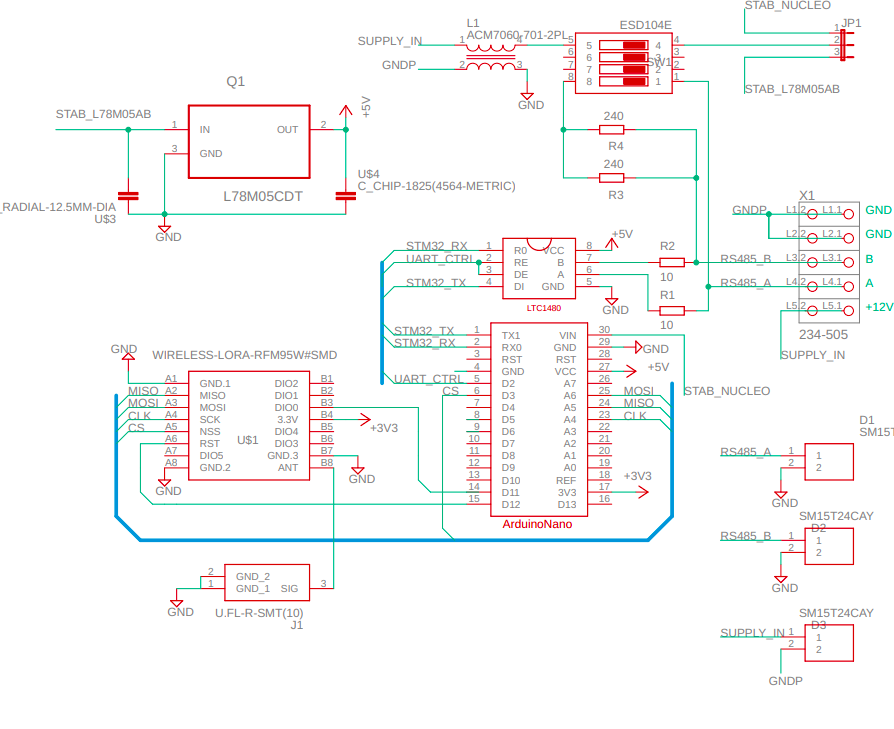
\includegraphics[width=1\textwidth]{minigateway_schema}
    \caption{Návrh gatewaye verze 2 - schéma}
    \label{fig:minigateway_schema}
\end{figure}

\begin{figure}[!h]
    \centering
    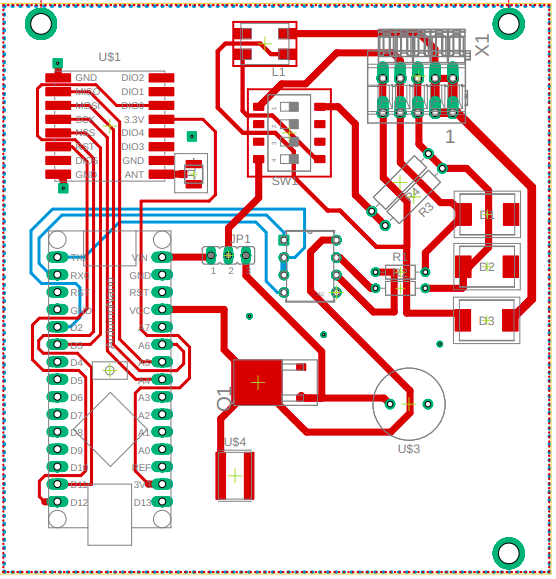
\includegraphics[width=0.7\textwidth]{minigateway_plosnak}
    \caption{Návrh gatewaye verze 2 - plošný spoj}
    \label{fig:minigateway_plosnak}
\end{figure}


Dle návrhu byla gateway realizována viz foto \ref{fig:minigateway_fotoV2}.

\begin{figure}[!h]
    \centering
    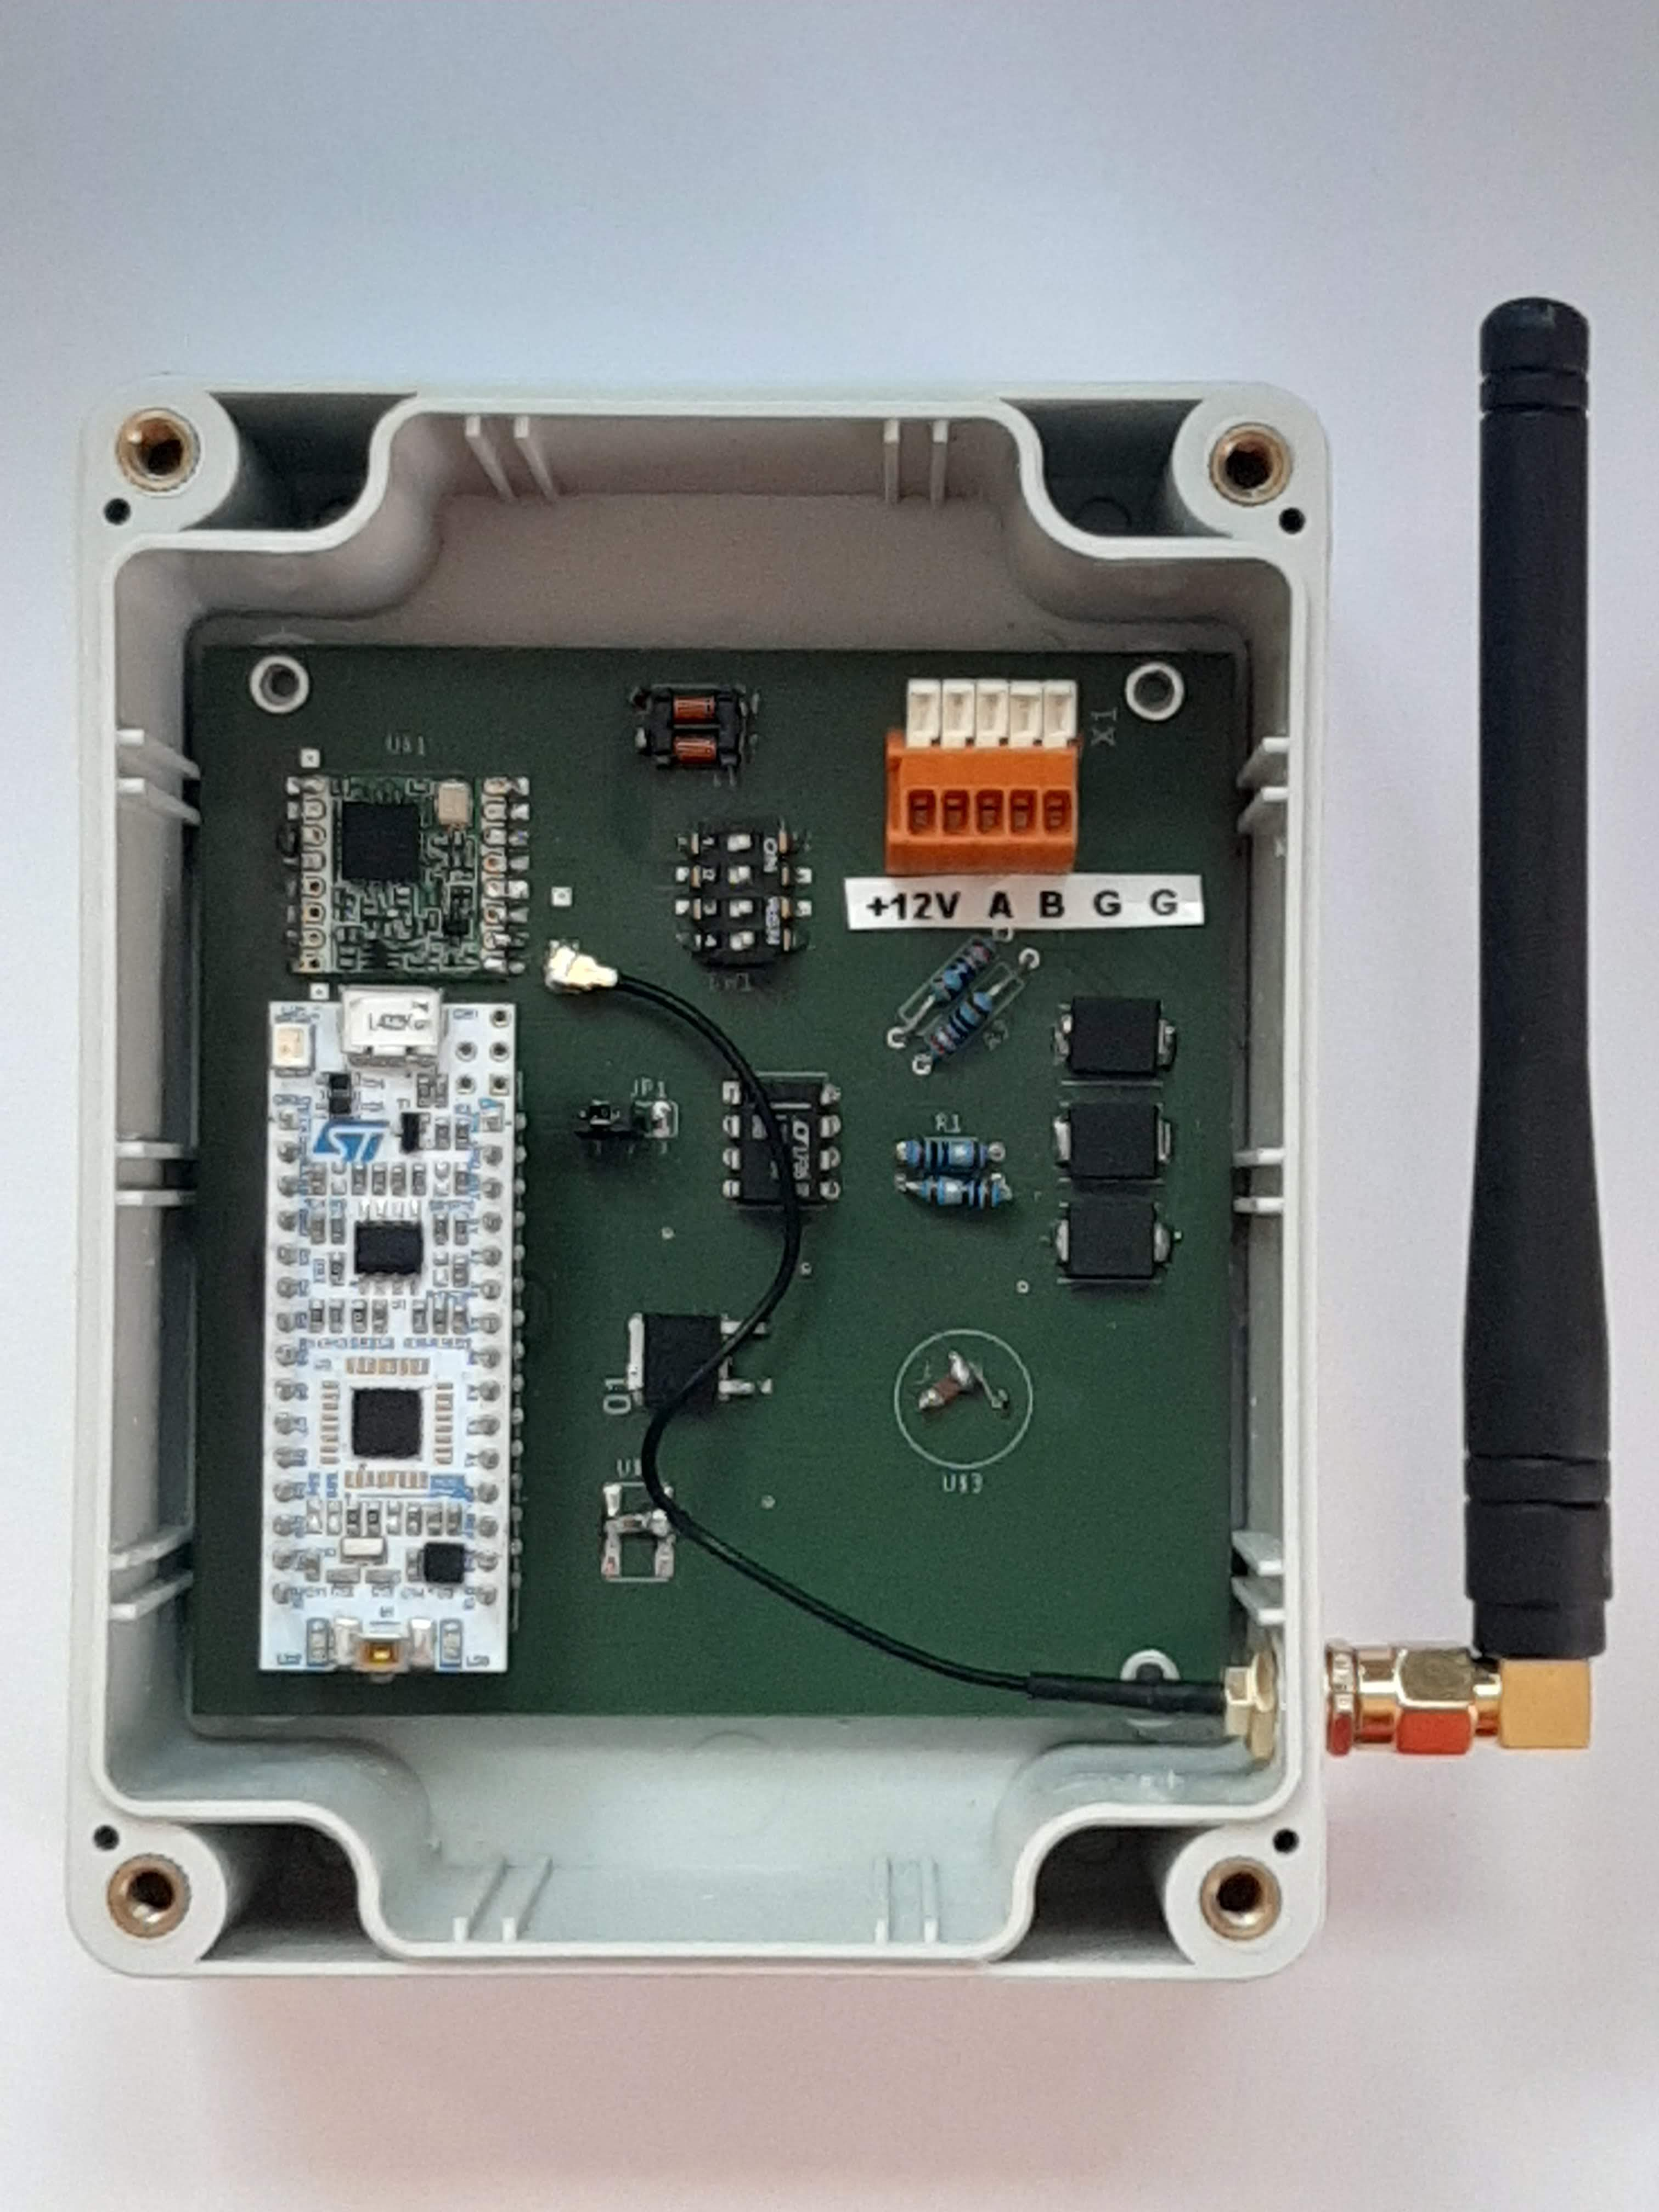
\includegraphics[width=0.6\textwidth]{photo_minigatewayV2}
    \caption{Foto gatewaye verze 2}
    \label{fig:minigateway_fotoV2}
\end{figure}



